\documentclass{beamer}

\usetheme{Copenhagen}
\definecolor{DALYellow}{RGB}{255, 212, 0}

\usepackage{tikz}
\usetikzlibrary{shapes,arrows}


% Define block styles
\tikzstyle{decision} = [draw, diamond, aspect=2, fill=blue!20]
\tikzstyle{block} = [rectangle, draw, fill=blue!20, text width=5em, text centered, rounded corners, minimum height=3em]
\tikzstyle{line} = [draw, -latex']
\tikzstyle{cloud} = [draw, ellipse, fill=red!20, node distance=3cm, minimum height=2em]
\tikzstyle{textyn} = [rectangle, text width=5em, text centered]

\beamertemplatenavigationsymbolsempty{}

% Set page number
\setbeamertemplate{page number in head/foot}[totalframenumber]

% ------------------
% Presentation title
% ------------------
\title[Weekly Meeting]{
    USRA Summer Weekly Meeting
}
\subtitle[]{Data Generation}
\author[Shuo Feng]{S. Feng}
\institute[NIMS Lab]{
  NIMS Lab\\
  USRA Summer 2023}
\date{\today}

\logo{
\includegraphics[height=1cm]{src/dal-logo-vm}}

\begin{document}

\frame{\titlepage}

\begin{frame}{Wrap-up: June 15 to June 20}

  Attempts:
  \begin{itemize}
    \item Get familiar with Slack and read the documentation for API
    \item Work on architecture issue (ARM and x86)
    \item Design automation process for Slack
  \end{itemize}

  Results:
  \begin{itemize}
    \item Working on writing scripts for Slack
    \item Abandon Kakao Talk or use a physical device
  \end{itemize}

\end{frame}

\begin{frame}{Capturing Process for Slack}
  \begin{center}
    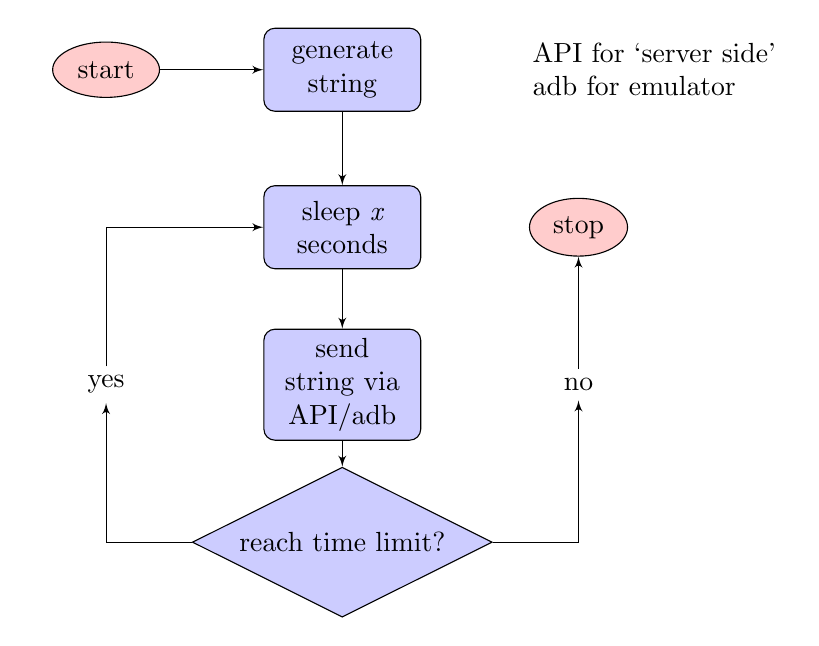
\begin{tikzpicture}[node distance = 2cm, auto]
      % Place nodes
      \node [block] (gen) {generate string};
      \node [cloud, left of=gen] (start) {start};
      \node [block, below of=gen] (sleep) {sleep \textit{x} seconds};
      \node [block, below of=sleep] (send) {send string via API/adb};
      \node [textyn, left of=send, node distance=3cm] (yes) {yes};
      \node [textyn, right of=send, node distance=3cm] (no) {no};
      \node [decision, below of=send] (decide) {reach time limit?};
      \node [cloud, right of=sleep, node distance=3cm] (stop) {stop};

      \node [right of=gen, node distance=4cm, text width=9em] (ex) {API for `server side' adb for emulator};

      % Draw edges
      \path [line] (gen) -- (sleep);
      \path [line] (sleep) -- (send);
      \path [line] (send) -- (decide);
      \path [line] (decide) -| (yes);
      \path [line] (yes) |- (sleep);
      \path [line] (decide) -| (no);
      \path [line] (no) -- (stop);
      \path [line] (start) -- (gen);
    \end{tikzpicture}
  \end{center}
\end{frame}

\begin{frame}{What to do next: June 22 to June 27}
  Schedule:
  \begin{itemize}
    \item Test capturing process for Slack
    \item Capture browsing traffic (Google Chrome)
    \item Capture traffic for Slack
  \end{itemize}

\end{frame}

\end{document}